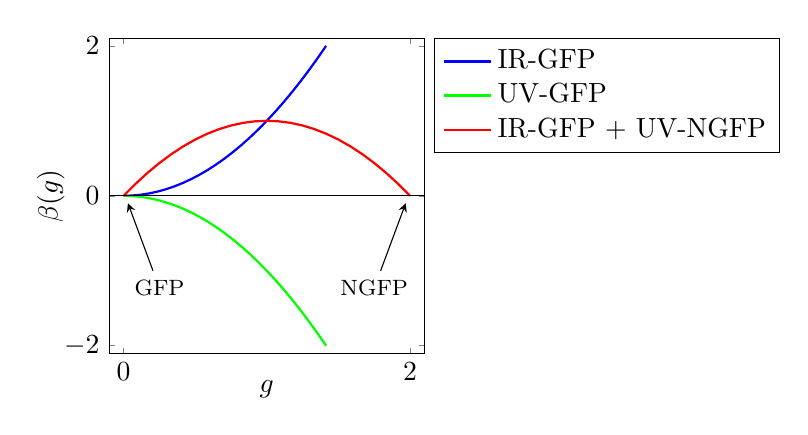
\begin{tikzpicture}[
    >=stealth,
    scale=1.00,
  ]

  \begin{axis}[
    width=4.0cm,
    height=4.0cm,
    scale only axis,
    major tick length=2pt,
    xlabel={$g$},
    ylabel={$\beta(g)$},
    xlabel shift=-7pt,
    ylabel shift=-7pt,
    xmin=-0.1, xmax=2.1,
    ymin=-2.1, ymax=2.1,
    xtick={0,2},
    ytick={-2,0,2},
    legend cell align=left,
    legend pos=outer north east,
    ]

    \addplot[blue,  domain=0:1.414, thick, ]{ x^2 };
    \addplot[green, domain=0:1.414, thick, ]{ - x^2 };
    \addplot[red,   domain=0:2.0, thick, ]{ 2*x - x^2 };
    \addplot[black, domain=-0.1:2.1, line width=0mm,  ]{ 0 };

    \legend{
      IR-GFP,
      UV-GFP,
      IR-GFP + UV-NGFP
    }


    \node (gfp) at (axis cs:0.25,-1.0) [anchor=north] {\footnotesize GFP};
    \draw[->] (gfp) -- (axis cs:0.03,-0.1);

    \node (ngfp) at (axis cs:1.75,-1.0) [anchor=north] {\footnotesize NGFP};
    \draw[->] (ngfp) -- (axis cs:1.97,-0.1);

  \end{axis}


\end{tikzpicture}
